{\fontsize{12}{14}\selectfont 

Il circuito utilizzato è costituito dall'elettrometro collegato al condensatore e dalla sfera conduttrice connessa a una delle uscite del generatore, posizionata ad almeno $50cm$ dal condensatore in modo che non sia presente una carica aggiuntiva dovuta ad un processo di induzione. 
\\
Il sistema formato dall'elettrometro e dal condensatore può essere schematizzato nel modo seguente:

\begin{figure}[H]
  \begin{minipage}[c]{0.4\textwidth}
    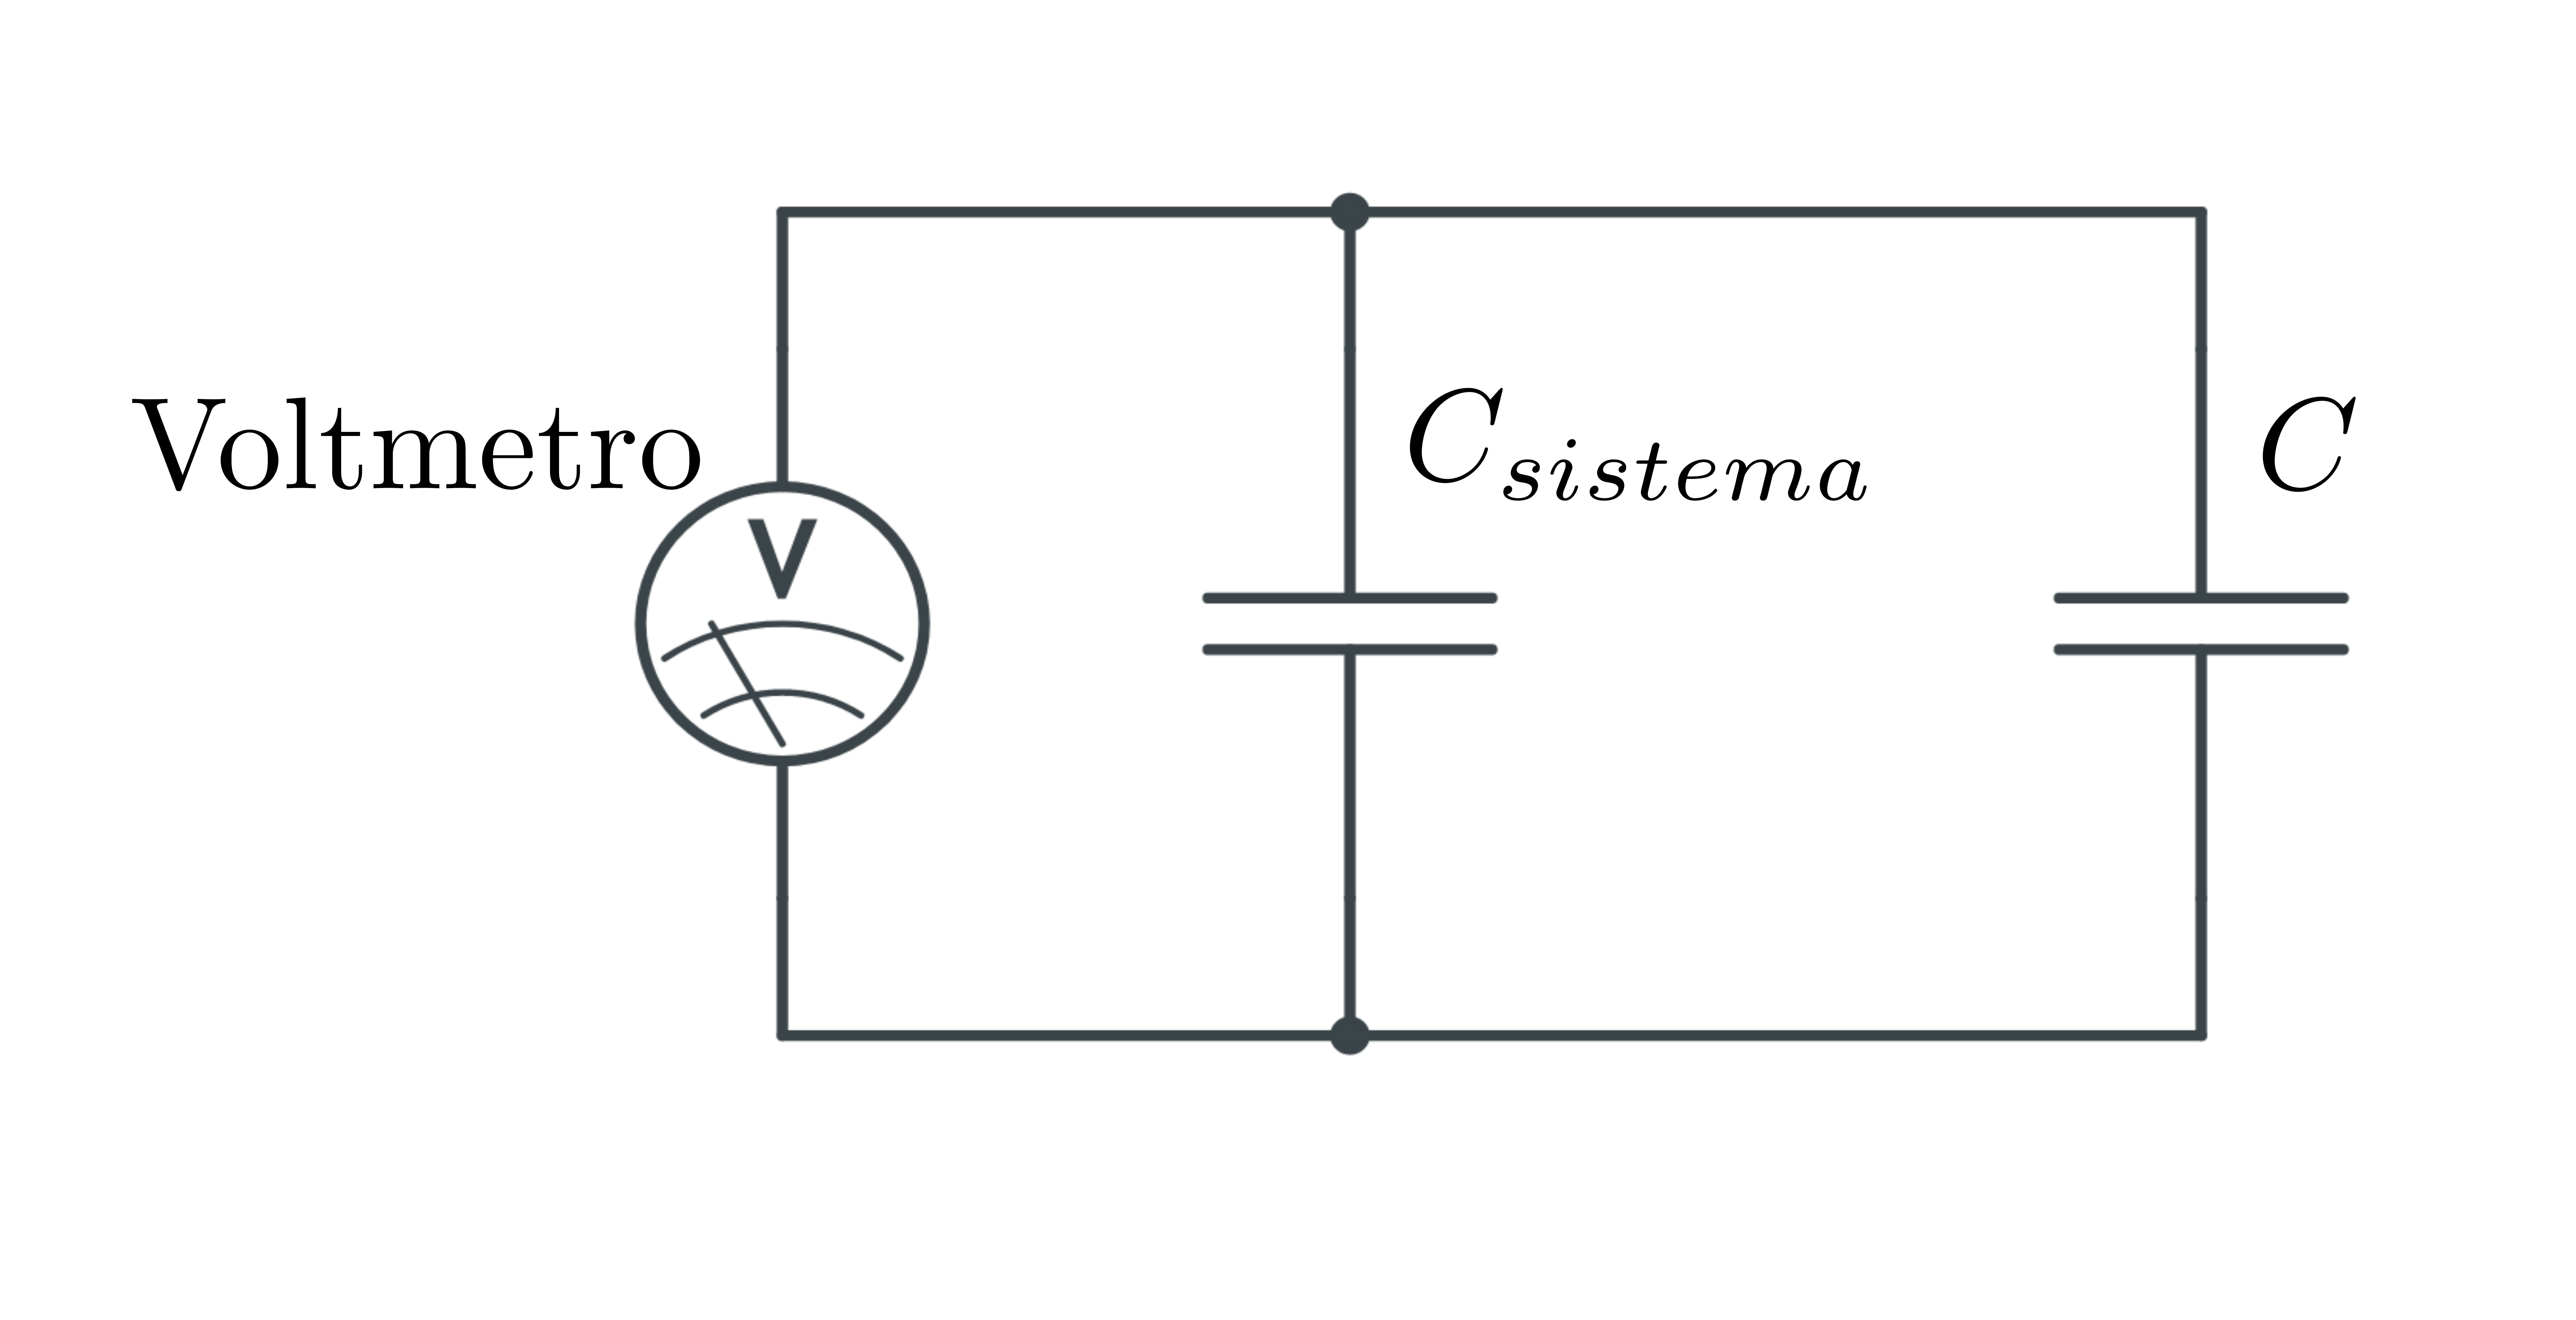
\includegraphics[width=8cm]{Figures/SchemaCircuitale3.png}
  \end{minipage}\hfill
  \begin{minipage}[c]{0.55\textwidth}
    \caption{
       Il circuito in figura mostra $C_{sistema}$ = capacità del sistema formato dall'elettrometro insieme ai suoi cavi, in parallelo con il condensatore $C$.
    } \label{fig:schemacircuitale}
  \end{minipage}
\end{figure}


Con la \emph{proof plane} è stata toccata prima la sfera e poi il condensatore per trasferire la carica, facendo in modo che le superfici fossero tangenti e che il contatto avvenisse sempre nello stesso punto. Dopo aver toccato il condensatore è stata rimossa la carica residua dalla \emph{proof plane} mettendola a contatto con la massa.

A diverse distanze tra le facce delle armature è stata trasferita la carica con $5$ tocchi ed è stata rilevata la misura della tensione con l'elettrometro.

Sono stati scelti 5 tocchi per sfruttare al meglio il fondoscala dell'elettrometro ed ottenere il miglior rapporto segnale/rumore.


Questo procedimento è stato ripetuto per sei diversi set di misura facendo variare al massimo un parametro alla volta:

\begin{enumerate}
    \item \textbf{Set$_1$} 3000V - 5 tocchi
    \item \textbf{Set$_2$} 3000V - 5 tocchi
    \item \textbf{Set$_3$} 3000V - 5 tocchi
    \item \textbf{Set$_4$} 2000V - 5 tocchi
    \item \textbf{Set$_5$} 3000V - 5 tocchi - 3s delay prima di trasferire la carica al condensatore
    \item \textbf{Set$_6$} 3000V - sfera a circa $12cm$ da un'armatura
\end{enumerate}

Sono state poi plottate le tensioni in funzione delle distanze ed è stato fatto un fit, prendendo in considerazione solo i punti fino a $d = 2 cm$, ovvero in approssimazione $d \ll \sqrt{A} = 15.8 cm$, usando la formula: 
\begin{equation*}
    V = \dfrac{Q}{\dfrac{\varepsilon A}{d} + C_{sistema}}
\end{equation*} 
che non può essere applicata in assenza di questa approssimazione.
\\
$\varepsilon$ è la costante dielettrica dell'aria uguale a $8.859 \cdot 10^{-12} \; C^2/(N \, m^2)$.
\\
$C_{sistema} = (113 \pm 30) pF$ come mostrato in appendice \ref{app:capacitasistema}.

Infine per stimare la carica totale $Q$ trasferita al condensatore si considera la sua capacità trascurabile rispetto a $C_{sistema}$ quando la distanza $d \geq 6 cm$, quindi si tracciano due rette asintotiche contenenti questi punti come mostrato nella \autoref{fig:parteIset1}. Queste rette rappresentano quei valori di tensione tali che 
\begin{equation*}
    V = \dfrac{Q}{C_{sistema}} 
\end{equation*}
e facendone la semisomma e la semidifferenza si è trovato, per ogni set, il valore di carica presente sul condensatore.

\par}